\documentclass[12pt]{letter}
\usepackage{amsmath,amsfonts,amsthm,amstext,amssymb,graphicx, multicol,fancyhdr,lastpage,fullpage,framed,fancybox,enumerate,tikz,color,mathrsfs, polynom}
\usepackage[margin=0.6in,headsep=3pt, headheight=15pt]{geometry}

% ----------------------------------------------------------
% Custom Definitions, Commands, Environments, etc.

% Sets of numbers
\def\R{\mathbb{R}} % The reals
\def\N{\mathbb{N}} % The naturals
\def\Z{\mathbb{Z}} % The integers
\def\Q{\mathbb{Q}} % The rationals

% Blank space
\newcommand{\blank}[1]{\underline{\hspace{#1}}} % Blank space

% Fitted inclusion symbols
\newcommand{\fp}[1]{\left({#1}\right)} % Fitted parentheses around content
\newcommand{\fb}[1]{\left[{#1}\right]} % Fitted brackets
\newcommand{\set}[1]{\left\{{#1}\right\}} % Fitted braces (useful for sets)
\newcommand{\av}[1]{\left|{#1}\right|} % Fitted absolute value bars

% Miscellaneous
\def\to{\rightarrow}
\def\then{\Rightarrow}



% Coordinate Plane (Four-Quadrant)
\def\coordplane {
	\begin{tikzpicture}		\draw[step=0.25cm,black,very thin,opacity=0.25] (-2.5cm, -2.5cm) grid (2.5cm, 2.5cm);
	\draw[<->,thick,black] (-2.5cm, 0) -- (2.5cm, 0) node[anchor=north west,pos=0.94,font=\scriptsize]{$x$};
	\draw[<->,thick,black] (0,-2.5cm) -- (0, 2.5cm) node[anchor=south east,font=\scriptsize,pos=0.94]{$y$};
	\end{tikzpicture}
}

% Coordinate Plane (One-Quadrant)
\def\onequad {
	\begin{tikzpicture}
	\draw[step=0.25cm, black, very thin, opacity=0.25] (0,0) grid (7.5cm,5cm);
	\draw[->, thick, black] (0,0) -- (7.5cm, 0) node[anchor=north west,font=\scriptsize,pos=0.94]{$x$};
	\draw[->, black, thick] (0,0) -- (0,5cm) node[anchor=south east,font=\scriptsize,pos=0.94]{$y$};
	\end{tikzpicture}
}

% Counters
\newcounter{exercise}

% Exercise environment (auto-numbered)
\newenvironment{exercise}[1][]{\begin{framed}\refstepcounter{exercise}\textbf{Exercise~\theexercise:} #1}{\end{framed}}

% Book exercise environment
\newenvironment{bex}[2][] {
	\begin{framed}
		\textbf{Book Exercise {#2}} #1
	\end{framed}
}
% ----------------------------------------------------------

\author{Jacob Ayers}

\begin{document}
	
	\textbf{Assignment 1 Key \\ MAT 130}
	
	\begin{bex}{P.1.8}
		{
			
		}
	\end{bex} \vspace{-8pt}
	
	% My answer here
	(a) $\set{12, 5}$ \\ (b) $\set{12, 5, 0}$ \\ (c) $\set{12, 5, 0, -7, -3}$ \\ (d) $\set{12, 5, 0, -7, -3, -\frac73, 3.14 \frac54}$ \\ (e) $\set{\sqrt{5}}$
	
	% \vspace{}
	\vfill % \newpage
	
	\begin{bex}{P.1.12}
		{
			
		}
	\end{bex}
	
	% My answer here
	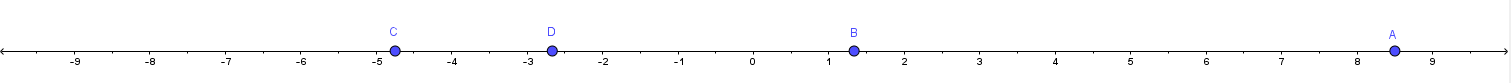
\includegraphics[width=\textwidth]{FigAnsP112.png}
	
	% \vspace{}
	 \vfill % \newpage
	
	\begin{bex}{P.1.20}
		{
			
		}
	\end{bex} \vspace{-8pt}
	
	% My answer here
	(a) The inequality represents all real numbers $x$ that are larger than $0$, and no more than $6$. \\
	(b) 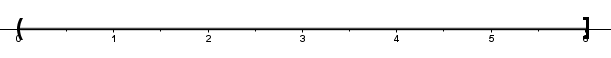
\includegraphics[width=0.5\textwidth]{FigAnsP120b.png} \\
	(c) This subset is bounded.
	
	% \vspace{}
	 \vfill % \newpage
	
	\begin{bex}{P.1.22}
		{
			
		}
	\end{bex} \vspace{-8pt}
	
	% My answer here
	(a) The inequality represents all real numbers that are less than $2$. \\
	(b) 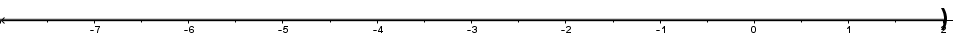
\includegraphics[width=0.5\textwidth]{P122b.png} \\
	(c) This subset is unbounded.
	
	% \vspace{}
	% \vfill % \newpage
	
	\begin{bex}{P.1.38}
		{
			
		}
	\end{bex} \vspace{-8pt}
	
	% My answer here
	If $x > 1$, then $\av{x - 1} = x - 1 >$. So $\dfrac{\av{x-1}}{x-1} = \dfrac{x - 1}{x - 1} = 1$.
	
	% \vspace{}
	 \vfill \newpage
	
	\begin{bex}{P.1.46}
		{
			
		}
	\end{bex} \vspace{-32pt}
	
	% My answer here
	\begin{flalign*}
	D &= \av{a - b} & \\
	&= \av{-\dfrac14 - \fp{-\dfrac{11}{4}}} & \\
	&= \av{\dfrac{10}{4}} & \\
	&= \dfrac{5}{2}
	\end{flalign*}
	
	% \vspace{}
	 \vfill % \newpage
	
	\begin{bex}{P.1.56}
		{
			
		}
	\end{bex} \vspace{-8pt}
	
	% My answer here
	Terms: $4x^3$, $0.5x$, $-5$ \\
	Coefficients: $4$, $0.5$
	
	% \vspace{}
	\vfill % \newpage
	
	\begin{bex}{P.1.60}
		{
			
		}
	\end{bex} \vspace{-8pt}
	
	% My answer here
	(a) $9 - 7(-3) = 7 + 21 = 30$ \\ (b) $9 - 7(3) = 9 - 21 = -12$
	
	% \vspace{}
	\vfill% \newpage
	
	\begin{bex}{P.1.64}
		{
			
		}
	\end{bex} \vspace{-8pt}
	
	% My answer here
	(a) $\dfrac{2 - 2}{2 + 2} = \dfrac{0}{4} = 0$ \\ (b) $\dfrac{-2 - 2}{-2 + 2)} = \dfrac{-4}{0}$, so the expression is undefined.
	
	% \vspace{}
	 \vfill %\newpage
	
	\begin{bex}{P.1.70}
		{
			
		}
	\end{bex} \vspace{-8pt}
	
	% My answer here
	$\dfrac{2x}{3} - \dfrac{x}{4} = \dfrac{8x}{12} - \dfrac{3x}{12} = \dfrac{5x}{12}$
	
	% \vspace{}
	 \vfill % \newpage
	
	\begin{bex}{P.2.12}
		{
			
		}
	\end{bex} \vspace{-8pt}
	
	% My answer here
	(a) $\dfrac{3}{3^{-4}} = 3^{1 - (-4)} = 3^5 = 243$ \\ (b) $48\fp{-4}^{-3} = \dfrac{48}{(-4)^3} = \dfrac{48}{-64} = -\dfrac{3}{4}$
	
	% \vspace{}
	 \vfill %\newpage
	
	\begin{bex}{P.2.16}
		{
			
		}
	\end{bex} \vspace{-8pt}
	
	% My answer here
	$7(4)^{-2} = 7\cdot\dfrac{1}{16} = \dfrac{7}{16}$
	
	% \vspace{}
	 \vfill \newpage
	
	\begin{bex}{P.2.20}
		{
			
		}
	\end{bex} \vspace{-8pt}
	
	% My answer here
	(a) $(5z)^3 = 5^3z^3 = 125z^3$ \\ (b) $5x^4(x^2) = 5x^6$
	
	% \vspace{}
	 \vfill % \newpage
	
	\begin{bex}{P.2.26}
		{
			
		}
	\end{bex} \vspace{-8pt}
	
	% My answer here
	(a) $\fb{\fp{x^2y^2}^{-1}}^{-1} = \fp{x^2y^2}^1 = x^2y^2$ \\ (b) $\fp{5x^2z^6}^3\fp{5x^2z^6}^{-3} = \dfrac{\fp{5x^2z^6}^3}{\fp{5x^2z^6}^3} = 1$
	
	% \vspace{}
	 \vfill % \newpage
	
	\begin{bex}{P.2.40}
		{
			
		}
	\end{bex} \vspace{-8pt}
	
	% My answer here
	(a) $3$ \\ (b) $216$
	
	% \vspace{}
	\vfill % \newpage
	
	\begin{bex}{P.2.42}
		{
			
		}
	\end{bex} \vspace{-8pt}
	
	% My answer here
	(a) $\sqrt{12}\cdot \sqrt{3} = \sqrt{36} = 6$ \\ (b) $\sqrt[4]{\fp{3x^2}^4} = 3x^2$
	
	% \vspace{}
	 \vfill % \newpage
	
	\begin{bex}{P.2.44}
		{
			
		}
	\end{bex} \vspace{-8pt}
	
	% My answer here
	(a) \vspace{-12pt} \begin{flalign*}
	\sqrt[3]{\dfrac{16}{27}} &= \dfrac{\sqrt[3]{16}}{\sqrt[3]{27}} & \\
	&= \dfrac{\sqrt[3]{8}\sqrt[3]{2}}{3} & \\
	&= \dfrac{2\sqrt[3]{2}}{3}
	\end{flalign*} \vspace{-12pt}
	(b) \begin{flalign*}
	\sqrt{\dfrac{75}{4}} &= \dfrac{\sqrt{75}}{\sqrt{4}} & \\
	&= \dfrac{\sqrt{25}\sqrt{3}}{2} & \\
	&= \dfrac{5\sqrt{3}}{2}
	\end{flalign*}
	
	% \vspace{}
	 \vfill \newpage
	
	\begin{bex}{P.2.54}
		{
			
		}
	\end{bex}
	
	% My answer here
	\vspace{-32pt} \begin{flalign*}
	\dfrac{3}{\sqrt{5} + \sqrt{6}}\fp{\dfrac{\sqrt{5} - \sqrt{6}}{\sqrt{5} - \sqrt{6}}} &= \dfrac{3\fp{\sqrt{5 - \sqrt{6}}}}{5 - \sqrt{30} + \sqrt{30} - 6} & \\
	&= \dfrac{3\fp{\sqrt{5} - \sqrt{6}}}{-1} & \\
	&= -3\fp{\sqrt{5} - \sqrt{6}}
	\end{flalign*}
	
	% \vspace{}
	\vfill % \newpage
	
	\begin{bex}{P.2.56}
		{
			
		}
	\end{bex} \vspace{-32pt}
	
	% My answer here
	\begin{flalign*}
	\dfrac{\sqrt{7} - 3}{4}\fp{\dfrac{\sqrt{7} + 3}{\sqrt{7} + 3}} &= \dfrac{7 + 3\sqrt{7} - 3\sqrt{7} - 9}{4\fp{\sqrt{7} + 3}} & \\
	&= -\dfrac{2}{4\fp{\sqrt{7} + 3}} & \\
	&= -\dfrac{1}{2\fp{\sqrt{7} + 3}}
	\end{flalign*}
	
	% \vspace{}
	 \vfill % \newpage
	
	\begin{bex}{P.2.62}
		{
			
		}
	\end{bex} \vspace{-8pt}
	
	% My answer here
	(a) $100^{-3/2} = \fp{\sqrt{100}}^{-3} = 10^{-3} = \dfrac{1}{1000}$ \\
	(b) $\fp{\dfrac94}^{-1/2} = \fp{\dfrac49}^{1/2} = \sqrt{\dfrac49} = \dfrac23$
	
	% \vspace{}
	\vfill % \newpage
	
	\begin{bex}{P.3.18}
		{
			
		}
	\end{bex} \vspace{-8pt}
	
	% My answer here
	$2x^2 + 1 - x^2 + 2x - 1 = x^2 + 2x$
	
	% \vspace{}
	 \vfill % \newpage
	
	\begin{bex}{P.3.22}
		{
			
		}
	\end{bex} \vspace{-8pt}
	
	% My answer here
	$15.6w^4 - 14w - 17.7 + 16.9w^4 - 9.2w + 13 = 32.5w^4 - 23.2w - 4.4$
	
	% \vspace{}
	 \vfill % \newpage
	
	\begin{bex}{P.3.34}
		{
			
		}
	\end{bex} \vspace{-8pt}
	
	% My answer here
	$x^2 + 4x - 8x - 32 = x^2 - 4x - 32$
	
	% \vspace{}
	\vfill % \newpage
	
	\begin{bex}{P.3.38}
		{
			
		}
	\end{bex}
	
	% My answer here
	\vspace{-32pt} \begin{flalign*}
	(2x^2 - x + 4)(x^2 + 3x + 2) &= 2x^4 + 6x^3 + 4x^2 - x^3 - 3x^2 - 2x + 4x^2 + 12x + 8 \\
	&= 2x^4 + 5x^3 + 5x^2 + 10x + 8
	\end{flalign*}
	
	% \vspace{}
	% \vfill \newpage
	
	\begin{bex}{P.3.42}
		{
			
		}
	\end{bex} \vspace{-8pt}
	
	% My answer here
	$u = 2x$, $v = 3$ \\
	$(u + v)(u - v) = u^2 - v^2$
	
	$(2x + 3)(2x - 3) = 4x^2 - 9$
	
	% \vspace{}
	\vfill % \newpage
	
	\begin{bex}{P.3.46}
		{
			
		}
	\end{bex} \vspace{-8pt}
	
	% My answer here
	$u = 8x$, $v = 3$ \\
	$(u + v)^2 = u^2 + 2uv + v^2$
	
	$(8x + 3)^2 = 64x^2 + 48x + 9$
	
	% \vspace{}
	% \vfill \newpage
	
	\begin{bex}{P.3.50}
		{
			
		}
	\end{bex}
	
	% My answer here
	$u = 3x$, $v = 2y$ \\
	$(u + v)^3 = u^3 + 3u^2v + 3uv^2 + v^3$
	
	$(3x + 2y)^3 = 27x^3 + 54x^2y + 36xy^2 + 8y^3$
	
	% \vspace{}
	\vfill % \newpage
	
	\begin{bex}{P.3.76}
		{
			
		}
	\end{bex} \vspace{-8pt}
	
	% My answer here
	Recall: The area of a triangle is found using the formula $A = \dfrac12 bh$
	\begin{flalign*}
	A_{\text{shaded}} &= A_{\text{large triangle}} - A_{\text{small triangle}} & \\
	&= \dfrac12 \fp{9x}\fp{12x} - \dfrac12 \fp{8x}\fp{6x} & \\
	&= 54x^2 - 24x^2 & \\
	&= 30x^2
	\end{flalign*}
	
	% \vspace{}
	 \vfill \newpage
	
	\begin{bex}{P.3.80}
		{
			
		}
	\end{bex}
	
	% My answer here
	(a) The height of the box has to be $x$, and the width is $15 - 2x$. Finding the length of the box is a little trickier. 
	
	Each short cut has a length of $x$ cm. If we let $y$ represent the length of the box, then $$3x + 2y = 45 \then y = -\dfrac32 x + \dfrac{45}{2}$$ Hence, \begin{flalign*}
	V &= \ell wh & \\
	&= \fp{-\dfrac32 x + \dfrac{45}{2}}\fp{15 - 2x}\fp{x} & \\
	&= \fp{-\dfrac32 x + \dfrac{45}{2}}\fp{15x - 2x^2} & \\
	&= 3x^3 - \dfrac{135}{2}x^2 + \dfrac{675}{2}x	
	\end{flalign*}
	(b) When $x = 3$: $3(3)^3 - 67.5(3)^2 + 337.5(3) = 486$ cm$^3$ \\
	When $x = 5$: $3(5)^3 - 67.5(5)^2 + 337.5(5) = 375$ cm$^3$ \\
	When $x = 7$: $3(7)^3 - 67.5(7)^2 + 337.5(7) = 84$ cm$^3$
	
	% \vspace{}
	 \vfill % \newpage
	
	\begin{bex}{P.4.14}
		{
			
		}
	\end{bex}
	
	% My answer here
	\vspace{-32pt} \begin{flalign*}
	81 - 36z^2 &= 9\fp{9 - 4z^2} & \\
	&= 9\fp{3 + 2z}\fp{3 - 2z}
	\end{flalign*}
	
	% \vspace{}
	\vfill % \newpage
	
	\begin{bex}{P.4.22}
		{
			
		}
	\end{bex} \vspace{-8pt}
	
	% My answer here
	$u = 6y$, $v = 7$ \\
	
	$36y^2 + 84y + 49 = (6y + 7)^2$
	
	% \vspace{}
	% \vfill \newpage
	
	\begin{bex}{P.4.26}
		{
			
		}
	\end{bex} \vspace{-8pt}
	
	% My answer here
	$u = x$, $v = 5$
	
	$x^3 + 125 = (x + 5)(x^2 - 5x + 25)$
	
	% \vspace{}
	\vfill  \newpage
	
	\begin{bex}{P.4.30}
		{
			
		}
	\end{bex} \vspace{-8pt}
	
	% My answer here
	$u = 4y$, $v = 5$
	
	$64y^3 - 125 = (4y - 5)(16y^2 + 20y + 25)$
	
	% \vspace{}
	 \vfill % \newpage
	
	\begin{bex}{P.4.36}
		{
			
		}
	\end{bex} \vspace{-8pt}
	
	% My answer here
	$(t - 3)(t + 2)$
	
	% \vspace{}
	 \vfill % \newpage
	
	\begin{bex}{P.4.40}
		{
			
		}
	\end{bex} \vspace{-32pt}
	
	% My answer here
	\begin{flalign*}
	8x^2 + 51x + 18 &= 8x^2 + 48x + 3x + 18 & \\
	&= 8x(x + 6) + 3(x + 6) & \\
	&= (8x + 3)(x + 6)
	\end{flalign*}
	
	% \vspace{}
	\vfill % \newpage
	
	\begin{bex}{P.4.46}
		{
			
		}
	\end{bex} \vspace{-32pt}
	
	% My answer here
	\begin{flalign*}
	3x^3 + x^2 - 15x - 5 &= x^2(3x + 1) - 5(3x + 1) & \\
	&= \fp{x^2 - 5}\fp{3x + 1}
	\end{flalign*}
	
	% \vspace{}
	\vfill % \newpage
	
	\begin{bex}{P.4.56}
		{
			
		}
	\end{bex} \vspace{-32pt}
	
	% My answer here
	\begin{flalign*}
	x^3 - 16x &= x\fp{x^2 - 16} & \\
	&= x(x+4)(x-4)
	\end{flalign*}
	
	% \vspace{}
	\vfill % \newpage
	
	\begin{bex}{P.4.60}
		{
			
		}
	\end{bex} \vspace{-32pt}
	
	% My answer here
	\begin{flalign*}
	9x^2 + 12x - 3x^3 &= -3x^3 + 9x^2 + 12x & \\ 
	&= -3x\fp{x^2 - 3x - 4} & \\
	&= -3x\fp{x-4}\fp{x+1}
	\end{flalign*}
	
	% \vspace{}
	% \vfill \newpage
	
	\begin{bex}{P.4.74}
		{
			
		}
	\end{bex} \vspace{-8pt}
	
	% My answer here
	$u = x$, $v = \dfrac34$
	
	$x^3 - \dfrac{27}{64} = \fp{x - \dfrac34}\fp{x^2 + \dfrac{3}{4}x + \dfrac{9}{16}}$
	
	% \vspace{}
	% \vfill \newpage
	
	
	
	
\end{document}